\documentclass{article}
%\copyrightyear{2012}
%\pubyear{2012}

\usepackage{listings}
\usepackage{multirow}
\usepackage{pdfpages}
\usepackage{color}
\def\Blah{\textit{Blah}\ }
\def\Gossamer{\textit{Gossamer}\ }
\def\Translucent{\textit{Translucent}\ }
\def\Trinity{\textit{Trinity}\ }
\def\Oases{\textit{Oases}\ }
\def\abinitio{\textit{ab initio}\ }
\def\denovo{\textit{de novo}\ }
\def\rhomer{$\rho$-mer\ }
\def\rhomers{$\rho$-mers\ }
\def\kmer{$k$-mer\ }
\def\kmers{$k$-mers\ }
\def\SQLite{\textit{SQLite}\ }
\newcommand{\jw}[1]{\marginpar{{\bf$\spadesuit$ JW}}{\bf #1}}
\newcommand{\js}[1]{\marginpar{{\bf$\clubsuit$ JS}}{\bf #1}}

\title{Visualising genome assemblies with \Blah}
\author{}
\begin{document}

\maketitle

\begin{abstract}
High throughput sequencing technologies can generate many millions of independent short reads which must then be organised in some way order to make sense of them.
A genome assembler is a tool for taking large sets of these reads and coalescing them into smaller sets of relatively long contiguous sequences (contigs.)
Although these contigs contain more contextual sequence information, simply by virtue of being longer, they must still be considered with respect to each other in order to understand the structure of the sampled genome. 
We describe \Blah, an web browser-based tool for visualising the result of genome assembly.
\Blah allows users to view graphs of contigs produced by an assembler, showing contigs' positions and orientations relative to each other, affording users a better understanding of the genome.
\textcolor{blue}{\Blah visualises a collection of contigs with respect to a reference genome by incorporating mapping information. This combination of information helps to establish genomic rearrangements with respect to the reference, such as copy number changes, inversions, transpositions, etc.
\Blah is an exploratory tool that aids the user in analysing specific regions of a target genome.}

\end{abstract}

\begin{figure}[t]
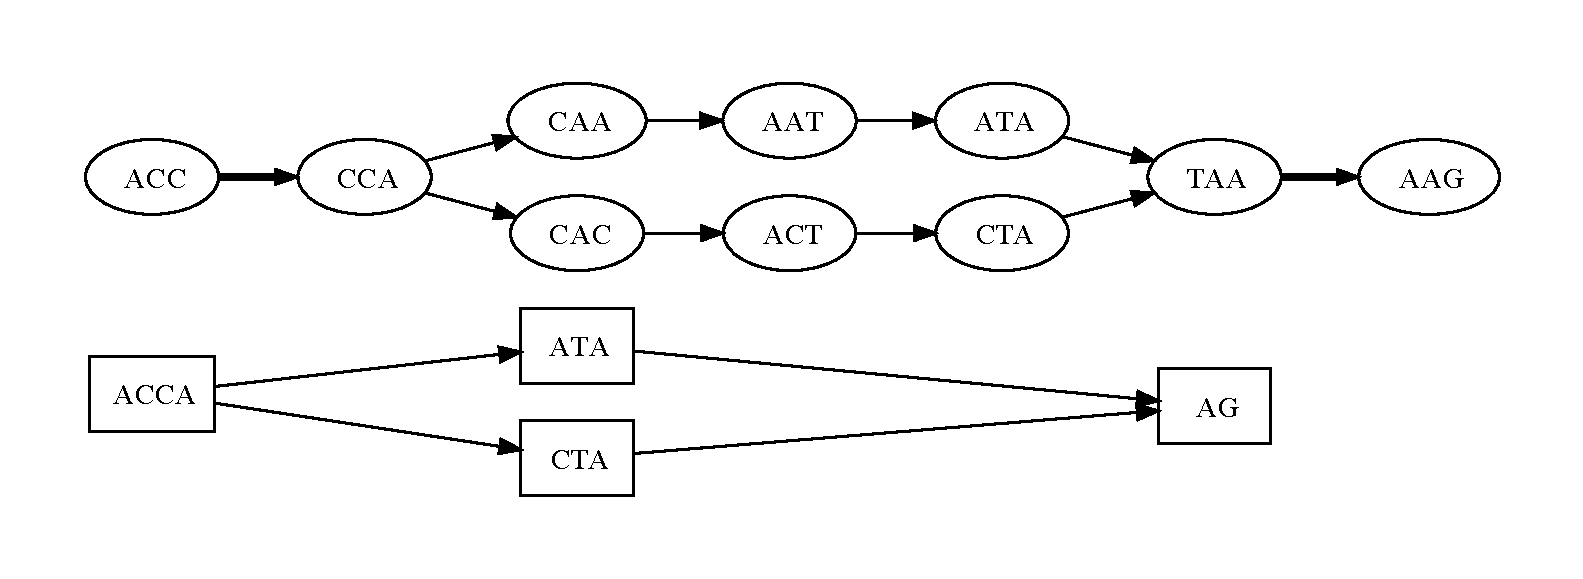
\includegraphics[width=\textwidth]{graph-k3.pdf}
\caption{de Bruijn graph (top) and corresponding contig graph (bottom) of two short sequences which differ by a single base pair.}
\label{fig:bubble}
\end{figure}

\section{Introduction}
Assembly provides a useful, unbiased way to analyse the genome of an organism. 
The process takes a large number of independent reads and produces a set of fewer, but much longer, sequences.
Although the result is a more manageable aggregation of all of those reads, we encounter some of the same problems 
when analysing the set of contigs, as we do when considering the original reads.
That is, the contigs appear as a set of independent sequences, without any structural context except for a notion of linkage between some contigs due to paired end information and split reads.

Assembly is mostly used as a de novo analysis tool of unknown sequence because of the unavailability of the more popular mapping approach (REF gossamer velvet etc).
However, assembly has a great advantage over mapping, that is, it is unbiased towards the input data: it does not try to press the analysed data into the framework of a reference genome, but merely associates reads that seem to be most similar.
Such lack of bias is particularly useful in sequencing data that is rather different from the available reference. 
When adding reference context after assembly (i.e. mapping the contigs to a reference), this bias is much less harmful, and genomic rearrangements can be interpreted more accurately (RESULT rather than statement).

Here we present \Blah as an graphical exploration device of de Bruijn graphs. 
It allows to investigate the structure of graphs (such as contig coverage or paired-end or split-read links between contigs) on any scale (user choses how much to display). 
Furthermore, \Blah has added functionality to incorporate reference genome context by incorporating mapping information of contigs and automatically aligning contigs on screen according to their genomic position.
Lastly, we added filtering tools that allow the user to search for likely points of interest in the graph -- such could be contigs that link to other contigs on different chromosomes (possible genomic rearrangements), contigs that link to other contigs with vastly different coverage (possible copy number changes), contigs that have strong links to more than one other contig (potential fusions, heterozygous rearrangements), etc.
The above features make \Blah useful in a de novo setting (exploration of CNVs, SVs, and assembly finish), as well as in a known organism (unbiased analysis of genomic rearrangements).

A common approach to assembly of high throughput sequencing data involves decomposing each read into all of its $k$ length substrings, i.e. \kmers.
The de Bruijn graph of this set of \kmers consists of a node for each \kmer and a directed edge from each node $a$ to node $b$ when $a$'s $k - 1$ suffix
is the same as $b$'s $k-1$ prefix.
Visualising the entire graph at once for even a small genome is impractical. 
For example, the graph of a typical \emph{Staphylococcus aureus} genome ($\sim$ 2.9 Mbp) contains 5,708,812 individual edges (at $k = 25$, and when including reverse complement edges). 
The majority of nodes have single incoming and outgoing edges, but even if we collapse such \emph{linear paths} of edges, the resulting graph still
contains 5,558 edges -- too many to lay out in a useful way.\jw{Perhaps we should use a human chromosome or even the whole genome for the example.} 
Consequently, to avoid presenting an overwhelming amount of data, a graph visualisation tool needs to allow users to focus on specific subgraphs to the exclusion of all else.

In general, it can be difficult for an assembler to resolve all ambiguities in the data.
Consider a diploid genome with a heterozygous SNP, and a sequencing process which yields all possible reads from that genome in equal proportions.
The \kmers drawn from those reads will come from either the sequences in common, immediately preceding and following the SNP, or will overlap the SNP.
The resulting de Bruijn graph structure, shown in Figure~\ref{fig:bubble} will contain a ``bubble'', and the assembler will output four separate contigs -- 
one for each linear path of edges.
From the contigs alone, we cannot reconstruct the original diagram, and have thus lost important positional information.

\section{Method}

%\begin{figure}
%{\small \tt
%\begin{tabular}{l}
%CREATE TABLE nodes (id INTEGER PRIMARY KEY ASC, rc INTEGER, cov\_mean REAL, length INTEGER);    \\
%CREATE TABLE links (id\_from INTEGER, id\_to INTEGER, gap INTEGER, count INTEGER, type INTEGER);        \\
%CREATE TABLE alignments (id INTEGER PRIMARY KEY ASC, name TEXT, start INTEGER, end INTEGER, matchLen INTEGER, dir INTEGER, gene TEXT);  \\
%CREATE TABLE sequences (id INTEGER PRIMARY KEY ASC, sequence TEXT);
%\end{tabular}
%\caption{Resource file SQL table schemas.}
%\label{fig:schemas}
%}
%\end{figure}

\begin{figure}
\setlength\fboxsep{0pt}
\fbox{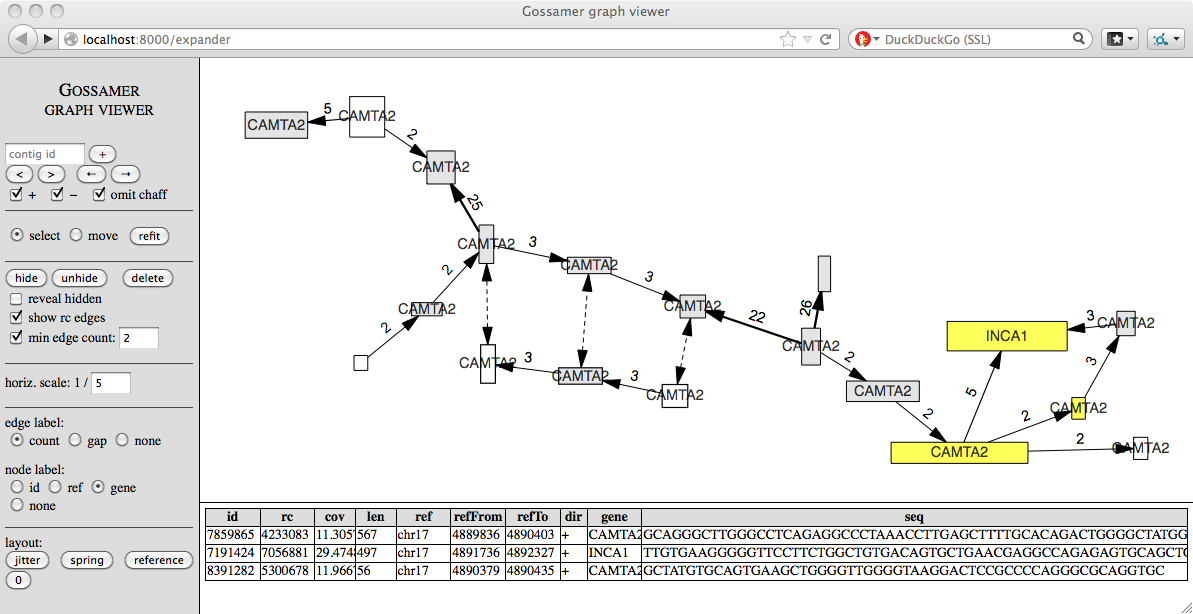
\includegraphics[width=\textwidth]{screenshot1.png}}
\caption{Screenshot of the \Blah graph viewer client.}
\label{fig:screenshot}
\end{figure}
\jw{better screenshot with less browser junk?}
\js{agree: something that shows the reference genome relation more clearly?}
The \Blah software consists of a web-based client -- the graph viewer application with which the user interacts -- and a server for supplying graph data on demand.
The server program is invoked with a database file which collects all information about the contigs and graph into a single place.

In \Blah, this resource file is simply an \SQLite database file containing a set of expected tables. 
%The table schemas are shown in Figure\ref{fig:schemas}.
In principle, any application or script could be used to produce an \SQLite database with the required tables: 
the contigs used could come form any assembler, and link information could be calculated from read pair alignments generated by a read mapping application.
To simplify the transition from an assembly result to a resource file for visualisation, we have extended the \Gossamer assembler with 
an additional command which causes it to generate an appropriate database file in a single invocation.

The viewer client is implemented in JavaScript, within a lightweight HTML document.
A screenshot of the viewer in use can be seen in Figure~\ref{fig:screenshot}.
The display window consists of three main panes: the control panel on the left; the graph view, which takes up most of the space; and a table of contig 
information, below the graph. 

Users begin by entering the id of a contig in the textbox in the upper left of the control panel, causing the contig's node to appear in the graph view. 
The upstream or downstream-linked neighbours of this, or any other node, can then be added by clicking on the $\leftarrow$ or $\rightarrow$ buttons, respectively.
If alignments are available, the $<$ and $>$ buttons will bring in the contig's immediate neighbours according to their alignments. 
In this way, the user is able to start at a promising contig, and then explore its context a step at a time.

As nodes are added, all edges incident to visible nodes are automatically added to the display. 
Additionally, double-ended, dotted arrows are drawn between pairs of contigs which are reverse complements.

The width of a node reflects the length of the underlying contig, while its height is a function of its mean coverage. 
i.e. longer contigs are wider, and higher coverage implies taller nodes.
The node's label can either be supressed, or set to its contig id, or if alignment information is present, its reference or gene name.
Edges can likewise be removed, or optionally labelled with either a count, e.g. the number of read pairs used to establish that link, 
or the genomic distance between the linked contigs, as represented by the edge.

Because not all nodes will be worth viewing at all times, users are free to hide (and then selectively reveal) nodes, or to delete them.
Note that only the display of the current subgraph is affected; the underlying graph is never manipulated.

Nodes in the graph view can be selected by clicking on them directly, or by dragging a selection box around them.
Selected nodes can then be manipulated as a group, i.e. moved, hidden, or deleted, and their key information viewed in the table at the bottom of the screen.
The contig table contains a row for each selected node, listing its: numeric id, the id of its reverse complement, mean coverage, length, optional 
reference alignment information (which reference and where), a possible gene name, if there is one and its known, and the contig base pair sequence itself.
Table headers can be clicked to sort all rows by the corresponding field.
Although often truncated, the sequence string is present in its entirety and can be selected and copied.

Three automatic layout algorithms are available at the click of a button.
If reference alignment information is present, nodes can be separated vertically into a series of rows -- one for each reference, e.g. human chromosome sequence -- 
and along those rows according to their relative alignment position.
Edges between nodes placed on different rows then represent links between different reference sequences. e.g. a potential inter-chromosomal rearrangement.
Also present is a spring-force based technique which tends to move closely linked nodes together while otherwise maintaining a degree of distance between all nodes.
Finally, the simplest ``layout'' algorithm simply randomly perturbs nodes' locations, useful for moving apart very near (or overlapping) nodes.

\textcolor{blue}{
\Blah's application is exploratory: the user can analyse a genomic region of interest or mine the contig information data base for interesting features, such as cross-chromosome links, or changes in contig coverage.
We implemented the following features to aid this process:
\begin{enumerate}
\item Location analysis: In the location search field (Figure XXX - Y) a genomic region can be entered; all contigs that fall into this region according to the mapping information are then displayed when clicking the Z button. All the features described above can then be applied to explore the region further.
\item Data base analysis: A few simple data mining steps can be applied to sort and filter the contig data base. For example, the user can list all contigs that align to different chromosomes of the reference genome, or sort the list of contigs by coverage, contig links, etc.
\end{enumerate}
}
\js{Realistic to implement such features? I think it would help the motivation of the whole thing significantly}

%\section{Discussion}

%\section*{Acknowledgement}
%
%National ICT Australia (NICTA) is funded by the Australian Government's Department of Communications; 
%Information Technology and the Arts;  
%Australian Research Council through Backing Australia's Ability; 
%ICT Centre of Excellence programs.

%\bibliographystyle{natbib}
\bibliographystyle{plain}
\bibliography{paper}

\end{document}
